%%%%%%%%%%%%%%%%%%%%%%%%%%%%%%%%%%%%%%%%%%%%%%%%%%%%%%%%%%%%%%%%%%%%%%%%%%%%%%%
\section{Test Cases and Reference Results}
\label{sec:test-cases}
%%%%%%%%%%%%%%%%%%%%%%%%%%%%%%%%%%%%%%%%%%%%%%%%%%%%%%%%%%%%%%%%%%%%%%%%%%%%%%%

This paper modeled two test cases derived from the Benchmark for Evaluation And Validation of Reactor Simulations (BEAVRS) PWR model \citep{horelik2013beavrs}. Each test case includes heterogeneous features -- and corresponding spatial self-shielding effects -- in order to understand their implications for accurate pin-wise MGXS generation. Although BEAVRS is an axially heterogeneous 3D core model, both benchmarks were fabricated in 2D due to the geometric constraints in OpenMOC. The impact of fuel enrichment, control rod guide tubes (CRGTs), burnable poisons (BPs), inter-assembly currents and water reflectors is considered. The geometric and material specifications for the two test cases are summarized in~\autoref{subsec:benchmarks}. The reference results computed with OpenMC are discussed in~\autoref{subsec:metrics}.


%%%%%%%%%%%%%%%%%%%%%%%%%%%%%%%%%%%%%%%%%%%%%%%%%%%%%%%%%%%%%%%%%%%%%%%%%%%%%%%
\subsection{Benchmark Configurations}
\label{subsec:benchmarks}

The two test cases were comprised of materials from the BEAVRS model, including 1.6\% and 3.1\% enriched UO$_2$ fuel, borated water (975 ppm boron), zircaloy, helium, air, borosilicate glass and stainless steel. The densities and isotopic compositions for each material are detailed in the BEAVRS specifications \citep{horelik2013beavrs}. Each material was modeled with cross sections from the ENDF/B-VII.1 continuous energy cross section library \citep{mcnpx2003manual} evaluated at 600K for hot zero power conditions.

The first benchmark was a single fuel assembly with an array of 264 fuel pins of 1.6\% enriched UO$_2$ fuel with zircaloy cladding and a helium gap. The assembly included 24 CRGTs filled by borated water and surrounded by zircaloy cladding, and a central instrument tube filled with air surrounded by two zircaloy tubes separated by borated water. The intra-pin grid spacer and grid sleeve separating each assembly in the BEAVRS model were not included in the assembly benchmark. The assembly was modeled with reflective boundary conditions. The fuel assembly benchmark is illustrated for null, degenerate and LNS homogenization in~\autoref{fig:benchmarks-assm}.

The second benchmark was constructed as a 2$\times$2 colorset of two fuel assemblies extracted from the BEAVRS model as illustrated in~\autoref{fig:null-reflector}. The top-left and bottom-right fuel assemblies were of the same enrichment and configuration as the single assembly benchmark. The top-right and bottom-left fuel assemblies included 264 fuel pins of 3.1\% enriched UO$_2$ fuel, 20 CRGTs and a central instrument tube. In addition, the two 3.1\% enriched assemblies included four BPs consisting of eight alternating layers of air, steel, borosilicate glass and zircaloy. The colorset was surrounded by a water reflector on the bottom and right that was of the same width as a fuel assembly, and was modeled with reflective boundaries on the top and left and vacuum boundaries on the bottom and right. The colorset is illustrated for null, degenerate and LNS homogenization in~\autoref{fig:benchmarks-colorset}.

\begin{figure*}[h!]
\centering
\begin{subfigure}{0.33\textwidth}
  \centering
  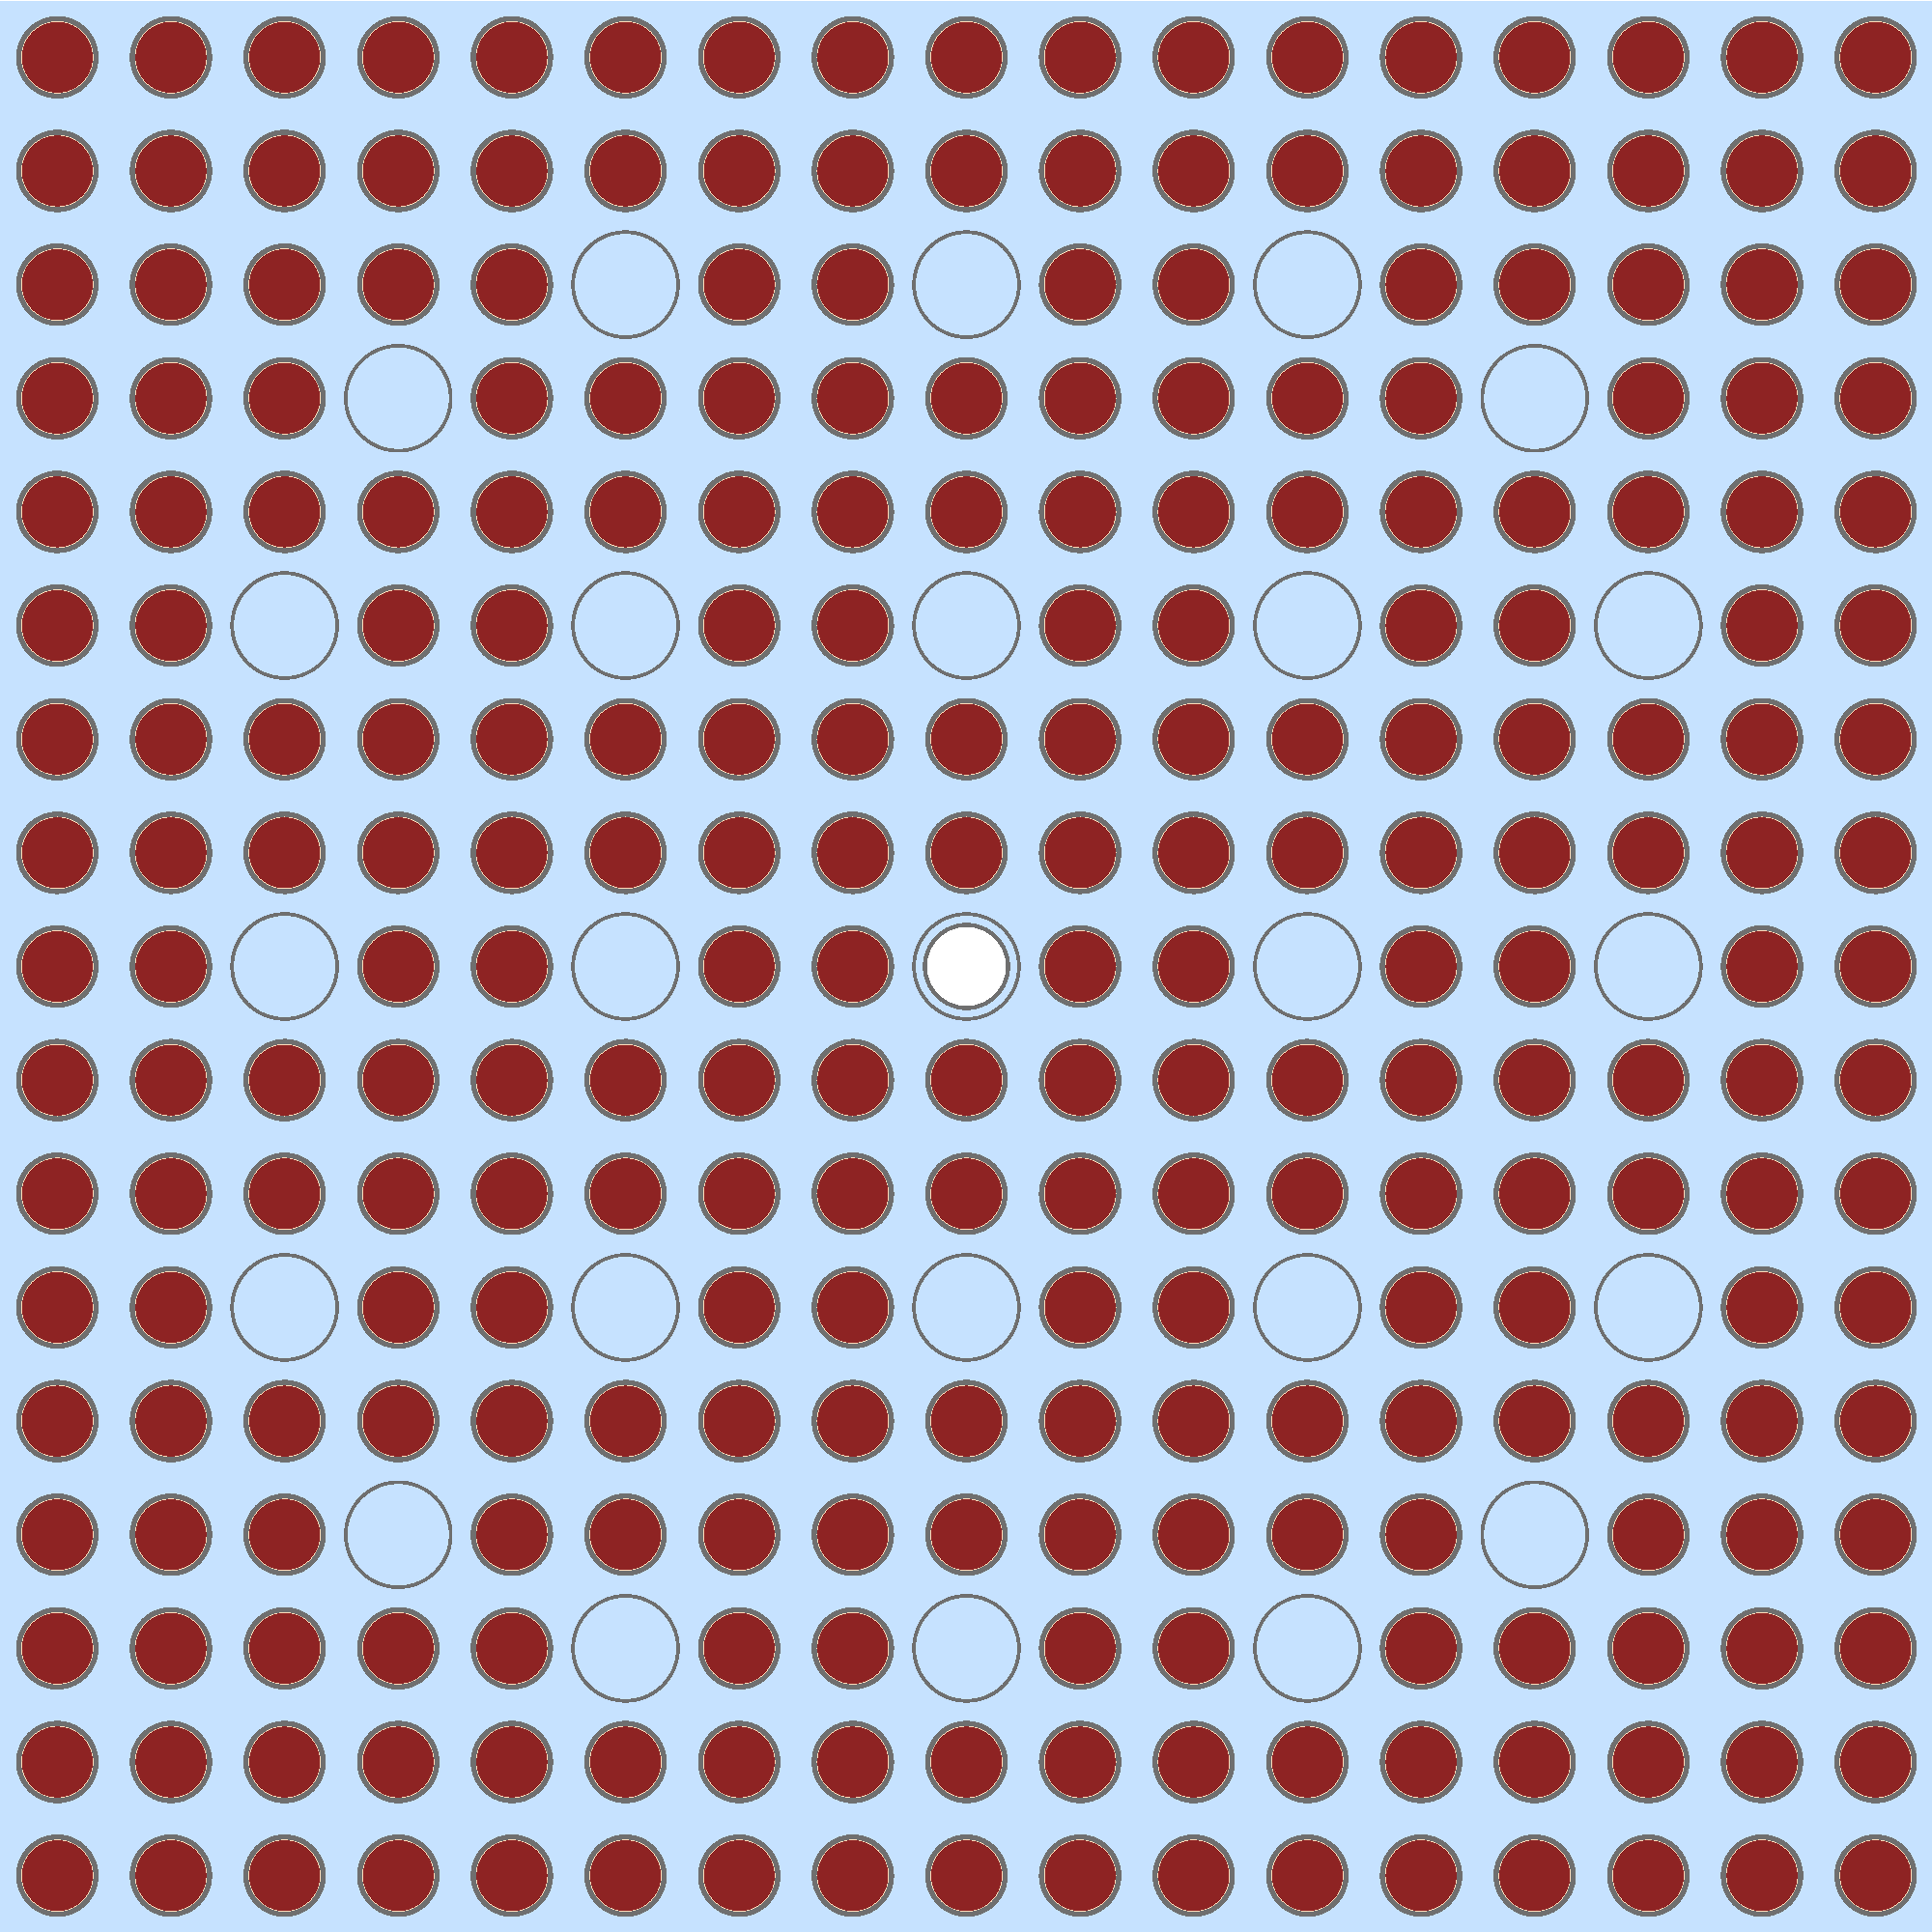
\includegraphics[width=0.9\linewidth]{figures/assembly/geometry}
  \caption{}
  \label{fig:null-assm}
\end{subfigure}
\begin{subfigure}{0.33\textwidth}
  \centering
  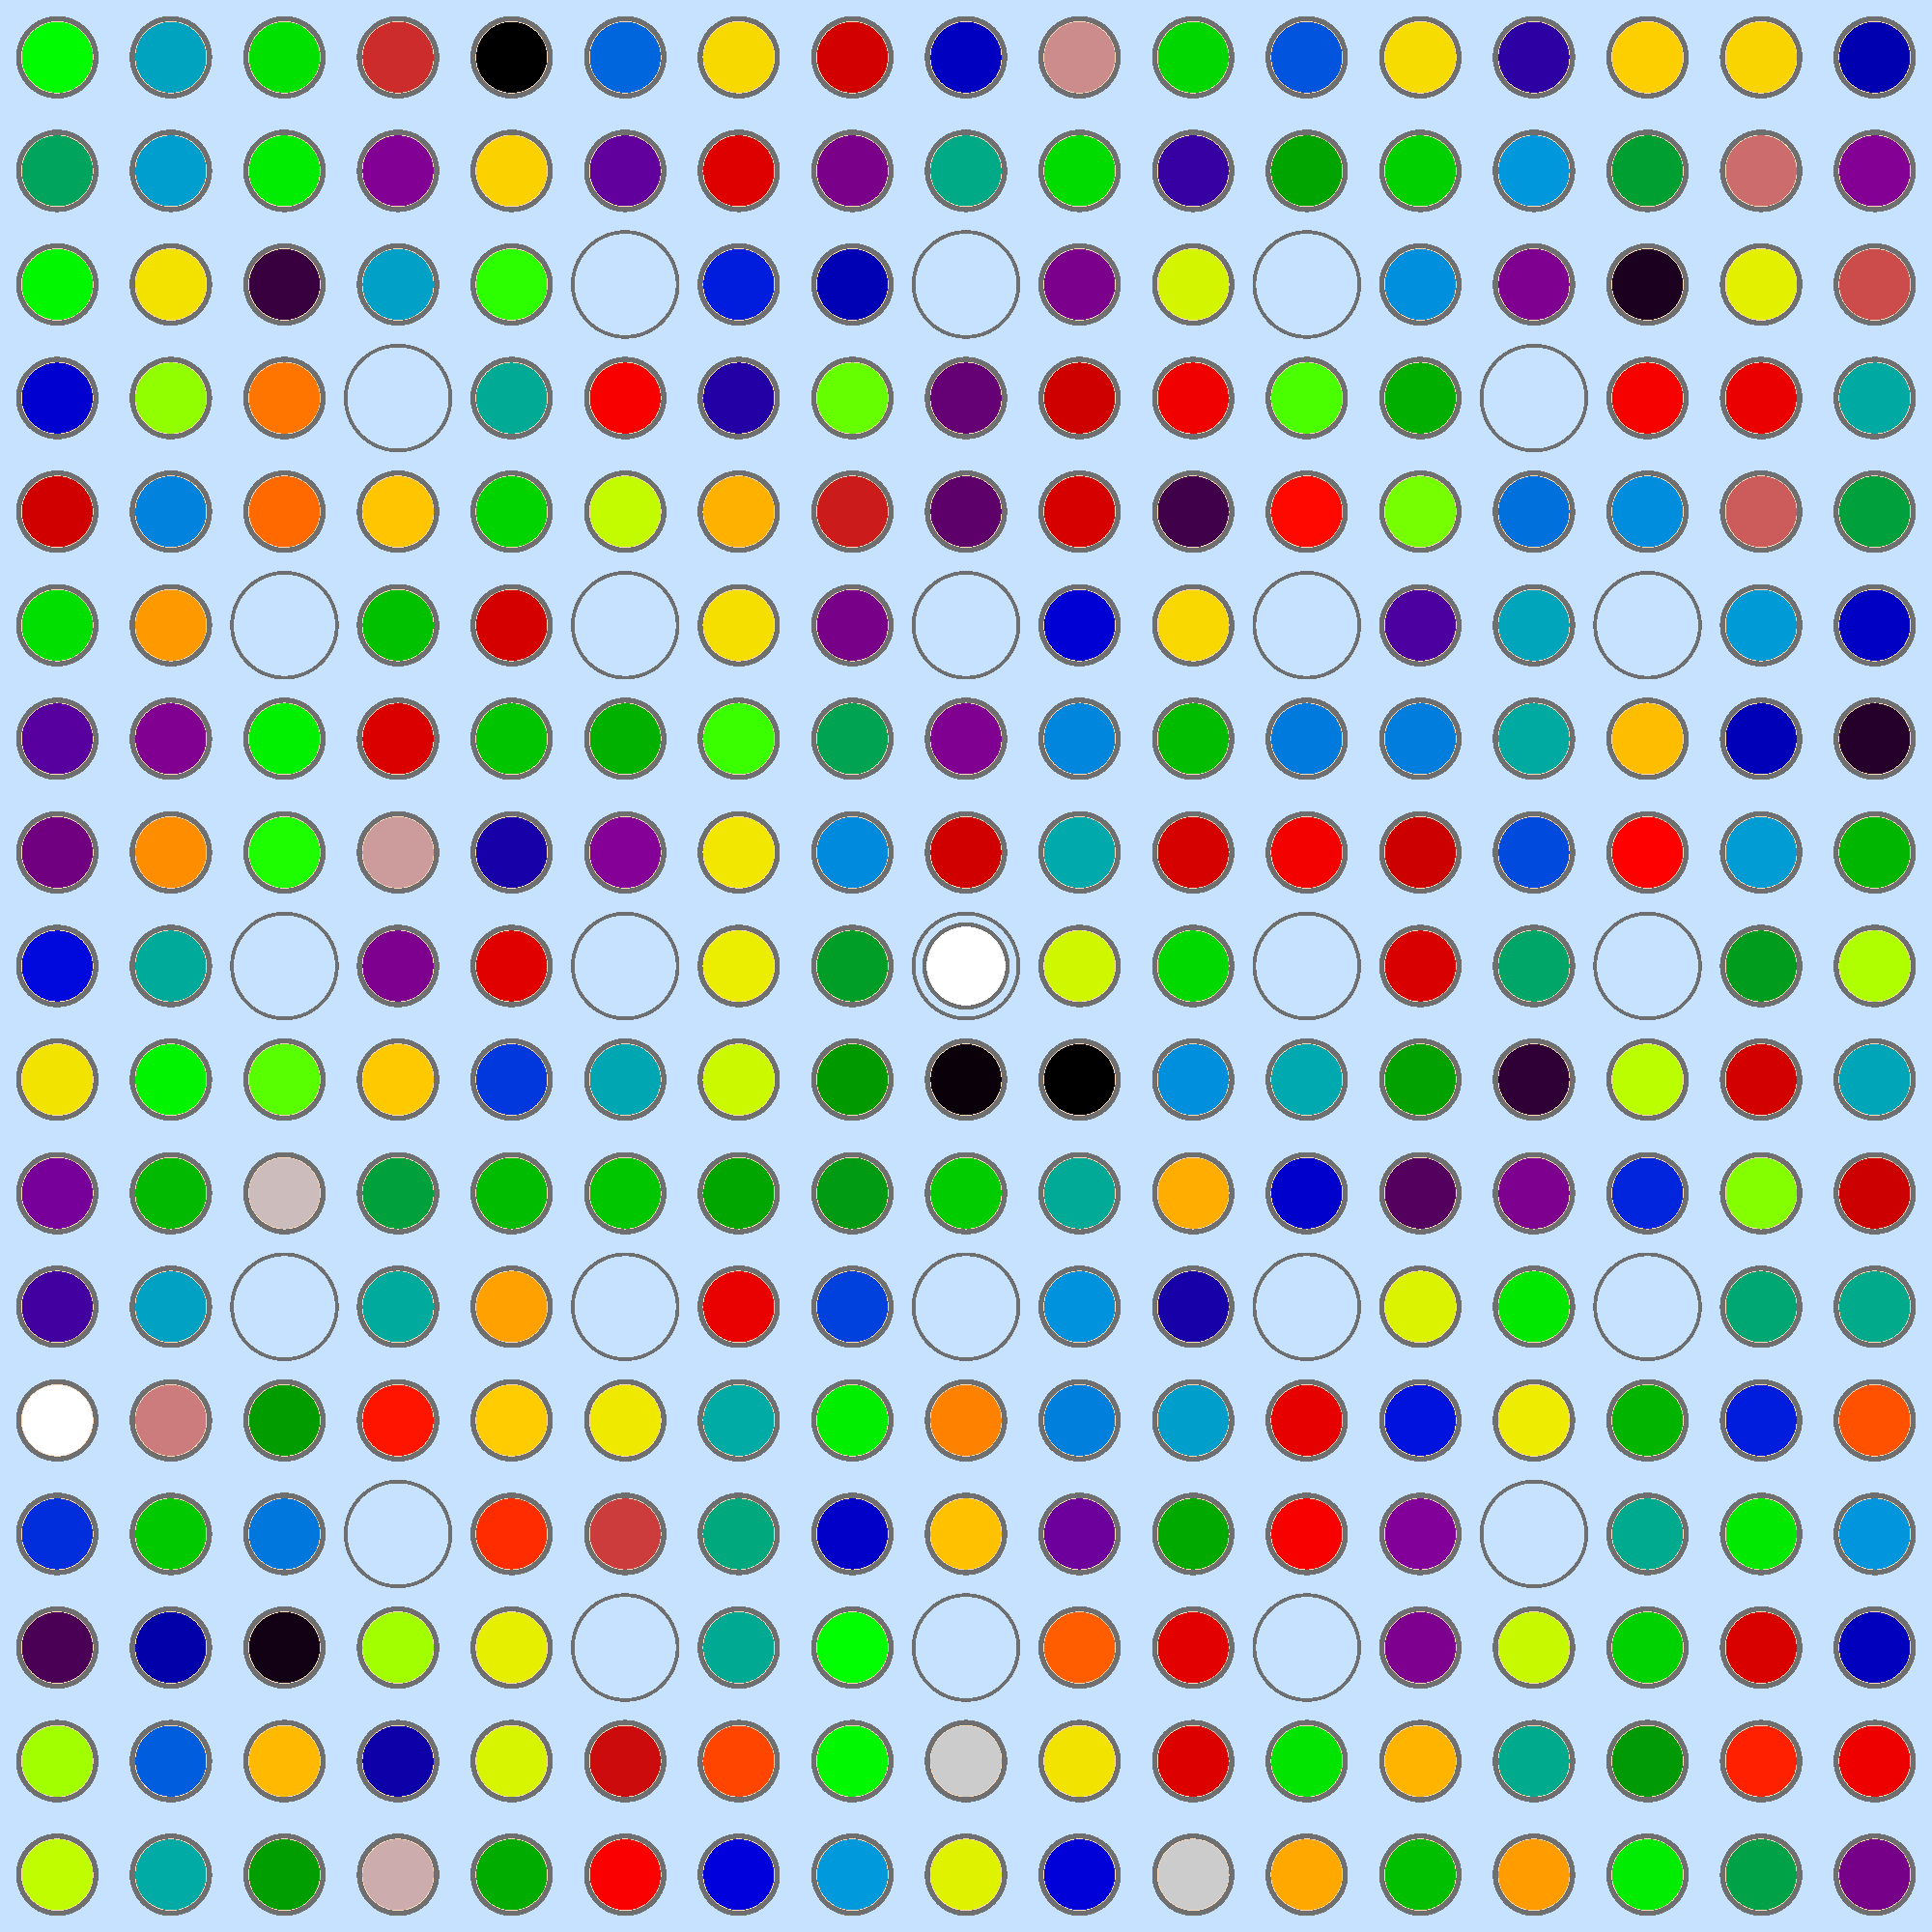
\includegraphics[width=0.9\linewidth]{figures/assembly/degenerate-materials}
  \caption{}
  \label{fig:degenerate-assm}
\end{subfigure}
\begin{subfigure}{0.33\textwidth}
  \centering
  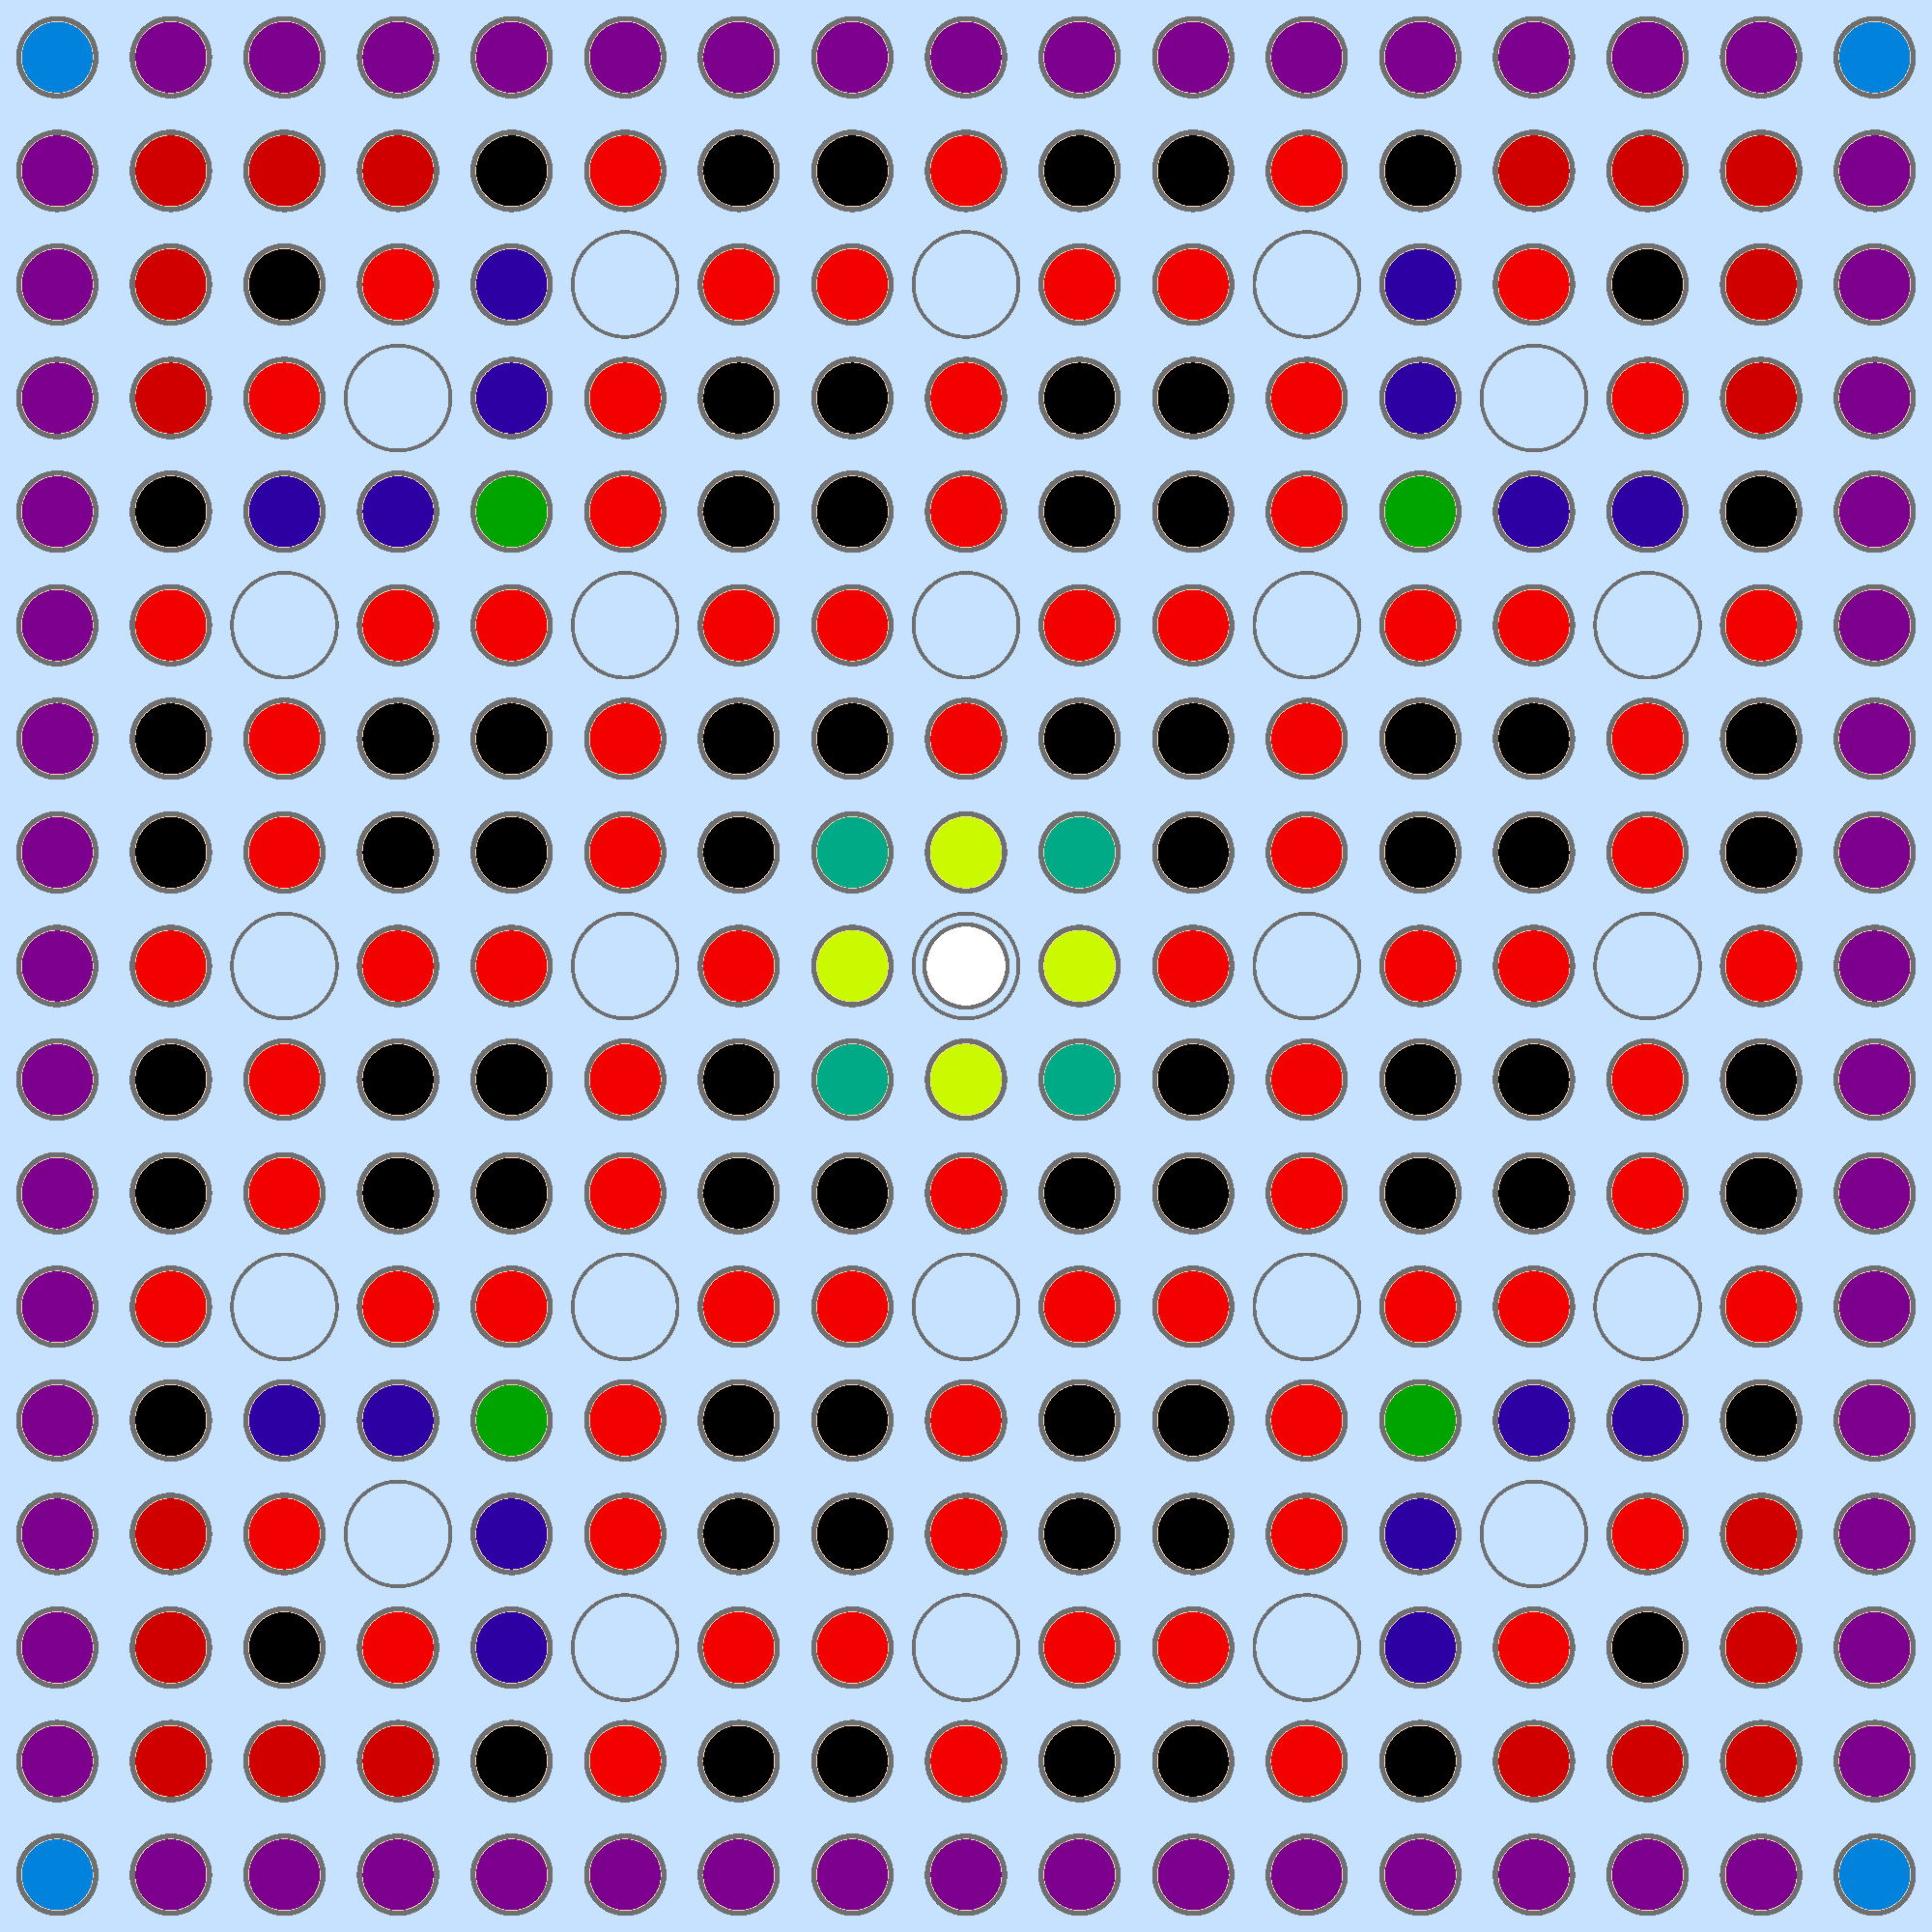
\includegraphics[width=0.9\linewidth]{figures/assembly/lns-materials}
  \caption{}
  \label{fig:lns-assm}
\end{subfigure}
\caption{OpenMOC materials for the assembly with null (a), degenerate (b) and LNS (c) homogenization.}
\label{fig:benchmarks-assm}
\end{figure*}

\begin{figure*}[h!]
\centering
\begin{subfigure}{0.33\textwidth}
  \centering
  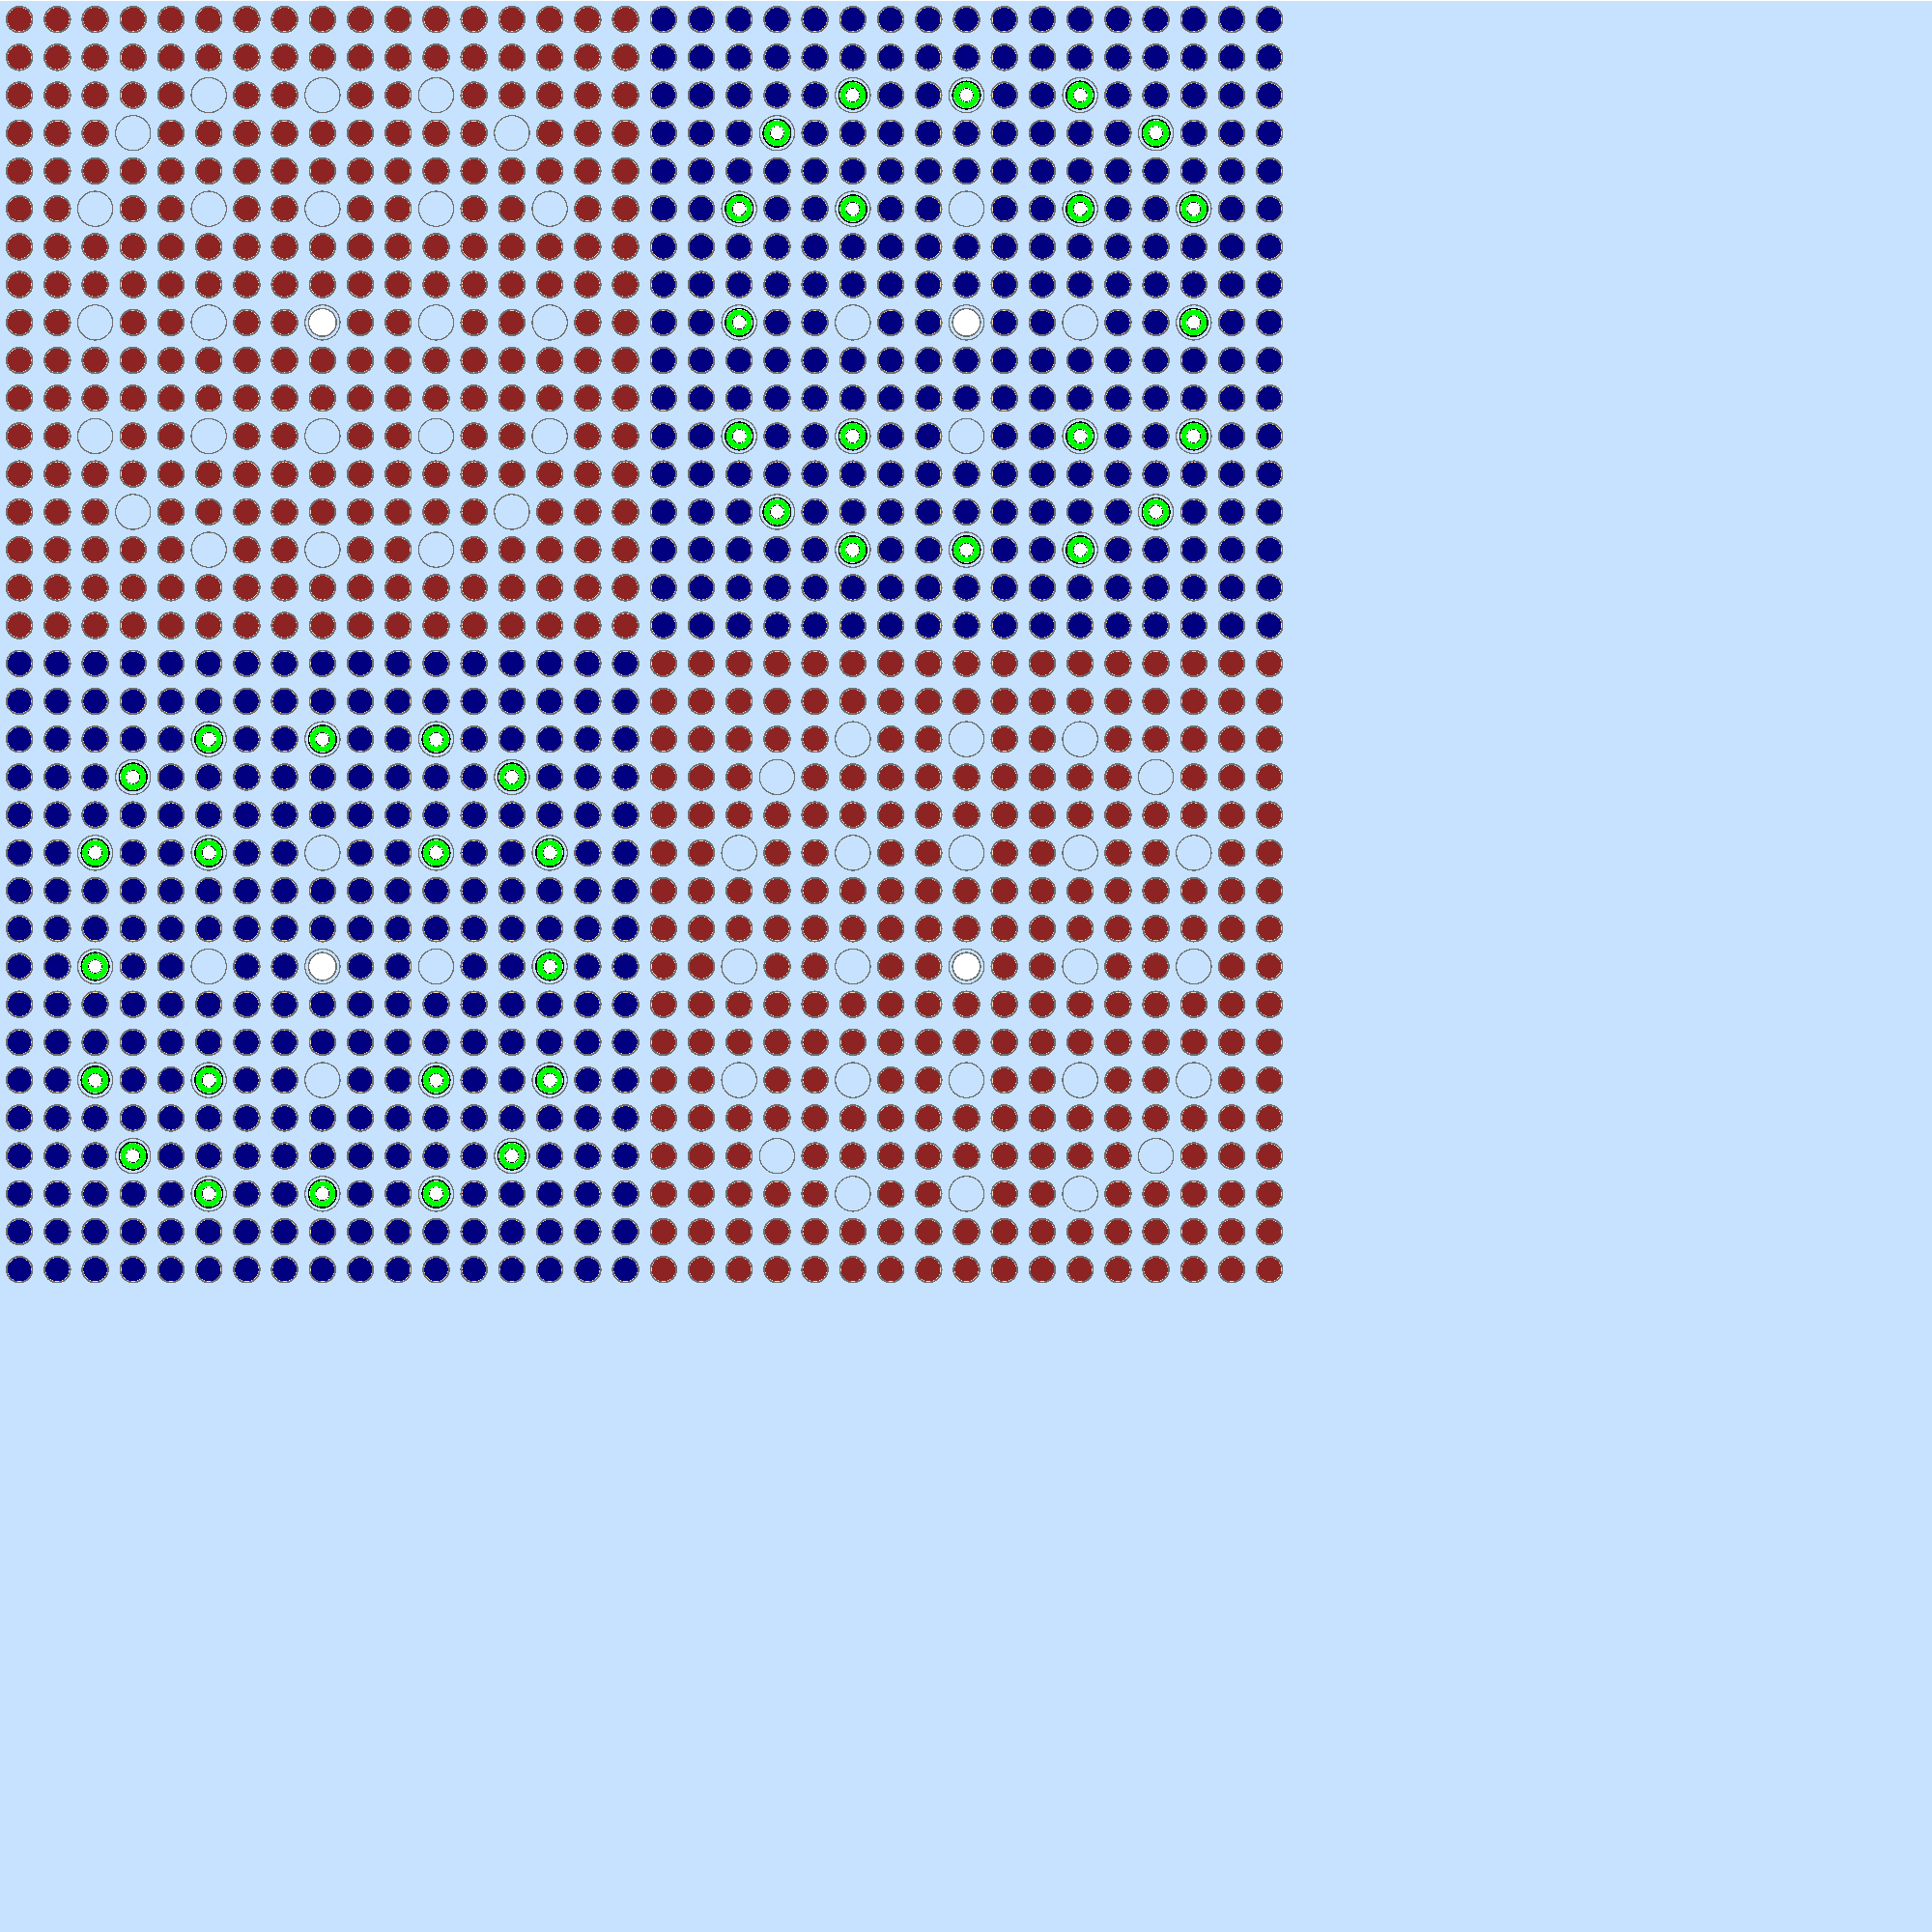
\includegraphics[width=0.9\linewidth]{figures/reflector/geometry}
  \caption{}
  \label{fig:null-reflector}
\end{subfigure}
\begin{subfigure}{0.33\textwidth}
  \centering
  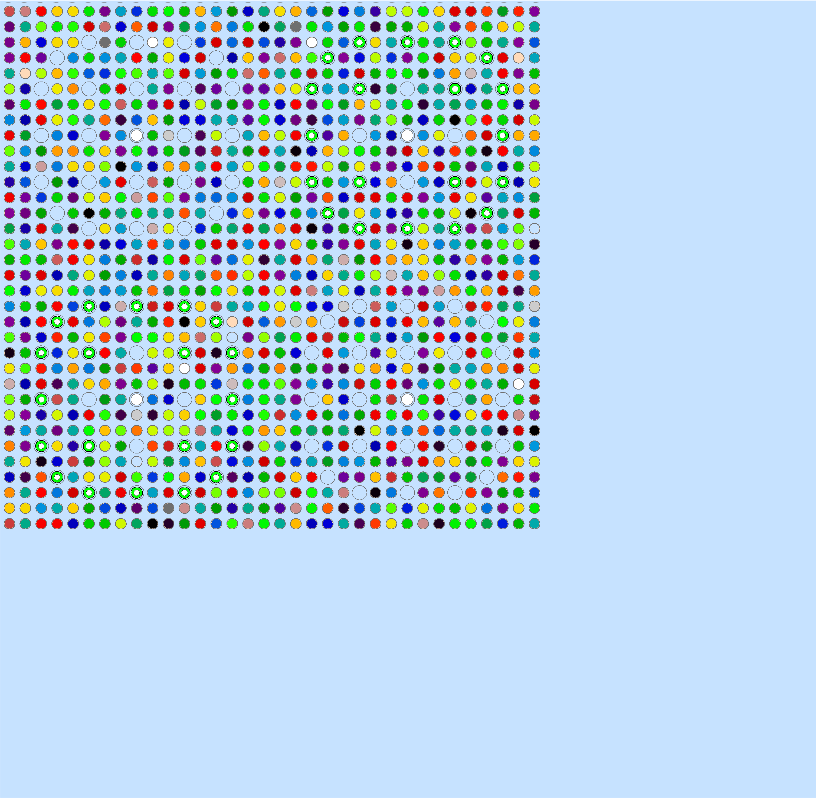
\includegraphics[width=0.9\linewidth]{figures/reflector/degenerate-materials}
  \caption{}
  \label{fig:degenerate-reflector}
\end{subfigure}
\begin{subfigure}{0.33\textwidth}
  \centering
  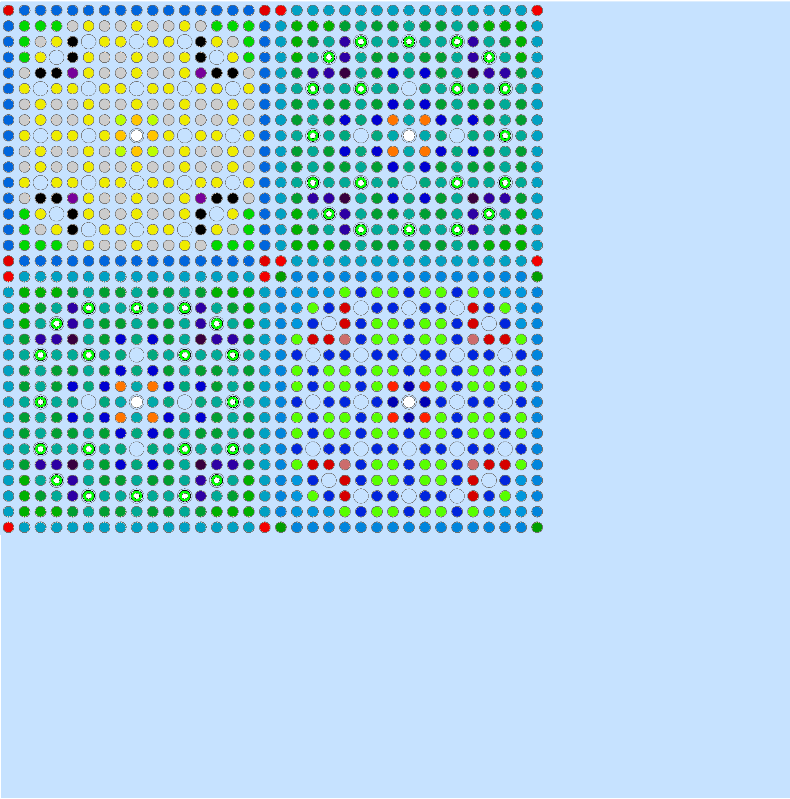
\includegraphics[width=0.9\linewidth]{figures/reflector/lns-materials}
  \caption{}
  \label{fig:lns-reflector}
\end{subfigure}
\caption{OpenMOC materials for the colorset with null (a), degenerate (b) and LNS (c) homogenization.}
\label{fig:benchmarks-colorset}
\end{figure*}

The fuel assembly and colorset benchmarks are color-coded by material and illustrated in \autoref{fig:lns-assm} and \autoref{fig:lns-reflector} for the LNS homogenization scheme. As indicated by the figures, fuel pin types with similar neighboring heterogeneities are assigned unique MGXS. As a result, LNS homogenization would be expected to enable more accurate predictions of reaction rate distributions than is possible with the null scheme. However, a cursory inspection of the colorset reveals a notable shortcoming of the LNS algorithm. In particular, the pins along the inter-assembly and assembly-reflector interfaces in the colorset are treated the same (\textit{i.e.}, with the same MGXS). As a result, LNS may result in poor reaction rate predictions for these pins. It is possible that the LNS algorithm could be specialized to differentiate between the pin types on the outer edge of each assembly, but such customizations would be challenging to implement and generalize.

The total number of materials (\textit{i.e.}, MGXS) used by each of the three homogenization schemes is given in \autoref{tab:num-materials-lns}. Only 9 -- 10 unique fissile materials are used for each fuel assembly with LNS, far fewer than the 264 in degenerate homogenization. Consequently, the MC tallies for LNS homogenization will converge more quickly than those for degenerate homogenization. 

\begin{table}[h!]
  \centering
  \caption{Number of fuel materials for each homogenization scheme.}
  \small
  \label{tab:num-materials-lns}
  \vspace{6pt}
  \begin{tabular}{l r r r}
  \toprule
  & \multicolumn{3}{c}{\bf \# Fuel Materials} \\
  \cline{2-4}
  \multirow{-2}{*}{\bf Benchmark} & \textbf{Null} & \textbf{Degenerate} & \textbf{LNS} \\
  \midrule
Assembly & 1 & 264 & 9 \\
Colorset & 2 & 1,056 & 29 \\
  \bottomrule
\end{tabular}
\end{table}

\begin{figure*}[h!]
\centering
\begin{subfigure}{0.42\textwidth}
  \centering
  
\includegraphics[width=0.8\linewidth]{figures/assembly/fsrs}
  \caption{}
  \label{fig:benchmarks-assm-fsrs}
\end{subfigure}%
\begin{subfigure}{0.42\textwidth}
  \centering
  
\includegraphics[width=0.8\linewidth]{figures/reflector/fsrs}
  \caption{}
  \label{fig:benchmarks-reflector-fsrs}
\end{subfigure}
\caption{OpenMOC FSRs for the assembly (a) and colorset (b) benchmarks.}
\label{fig:benchmarks-fsrs}
\end{figure*}


%The colorset does not include the stainless steel baffle surrounding the fuel assemblies adjacent to the water reflector in the full core BEAVRS model.

Flat source region spatial discretization meshes were applied to both benchmarks for the OpenMOC simulations as shown in~\autoref{fig:benchmarks-fsrs}. The UO$_2$ fuel was subdivided into five equal volume radial rings, while ten radial rings were employed in the water-filled CRGTs and instrument tubes. The borosilicate glass and borated water material zones filling the BPs were each discretized into five equal volume radial rings. Five equally spaced rings were used in the moderator zones surrounding each pin. Eight equal angle subdivisions were used in all pin cell material zones. The 13.85824 cm of water reflector nearest the fuel assemblies in the colorset benchmark was discretized in a 0.125984 cm $\times$ 0.125984 cm rectilinear mesh, equivalent to a 10$\times$10 mesh in each pin. The 7.55904 cm of reflector furthest from the fuel assemblies was discretized in a 1.25984 cm $\times$ 1.25984 cm pin-wise mesh.

%%%%%%%%%%%%%%%%%%%%%%%%%%%%%%%%%%%%%%%%%%%%%%%%%%%%%%%%%%%%%%%%%%%%%%%%%%%%%%%
\subsection{Verification Metrics}
\label{subsec:metrics}

A series of OpenMC simulations was used to calculate reference eigenvalues, pin-wise fission rates, and pin-wise U-238 capture rates for both benchmarks. A factor of 10$\times$ more particle histories per batch (\textit{i.e.}, 10$^7$ per batch) were used for the reference calculations relative to the OpenMC simulations used to generate MGXS. The OpenMC ``combined'' eigenvalue estimator is reported along with the associated 1-sigma uncertainty of one pcm for both benchmarks in~\autoref{tab:keff-reference}.

% The reference solutions were computed with 100 inactive and 900 active batches of 10$^7$ particle histories per batch.

\begin{table}[h!]
  \centering
  \caption{Reference OpenMC eigenvalues for each benchmark.}
  \label{tab:keff-reference} 
  \begin{tabular}{c c}
  \toprule
  {\bf Assembly} &
  {\bf Colorset} \\
  \midrule
  0.99326 $\pm$ 0.00001 & 0.94574 $\pm$ 0.00001 \\
  \bottomrule
\end{tabular}
\end{table}

\begin{figure*}[h!]
\centering
\begin{subfigure}{0.4\textwidth}
  \centering
  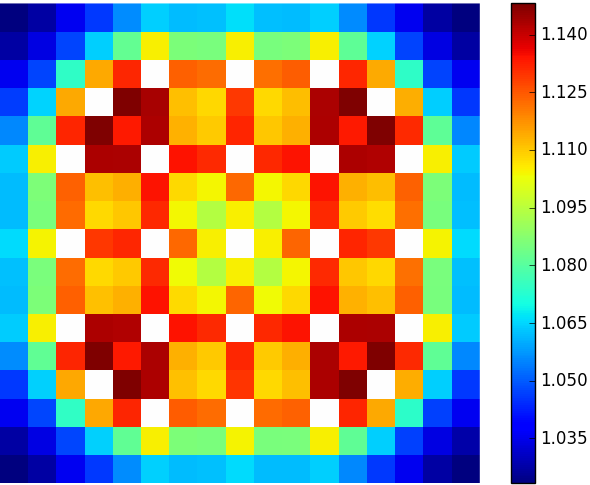
\includegraphics[width=0.8\linewidth]{figures/assembly/fission-rates}
  \caption{}
  \label{fig:fiss-assm}
\end{subfigure}%
\begin{subfigure}{0.4\textwidth}
  \centering
  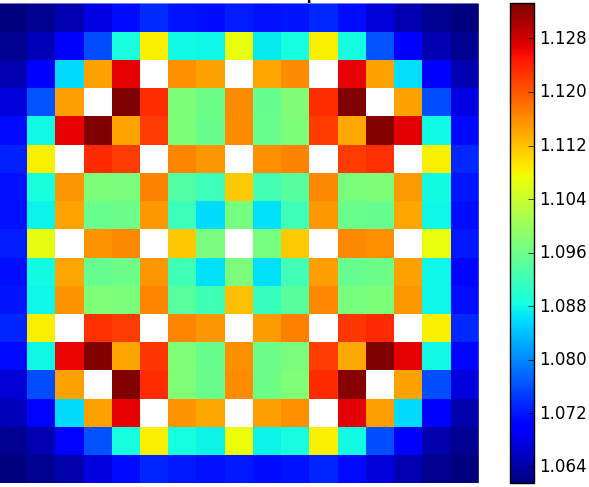
\includegraphics[width=0.8\linewidth]{figures/assembly/capture-rates}
  \caption{}
  \label{fig:capt-assm}
\end{subfigure}
\begin{subfigure}{0.4\textwidth}
  \centering
  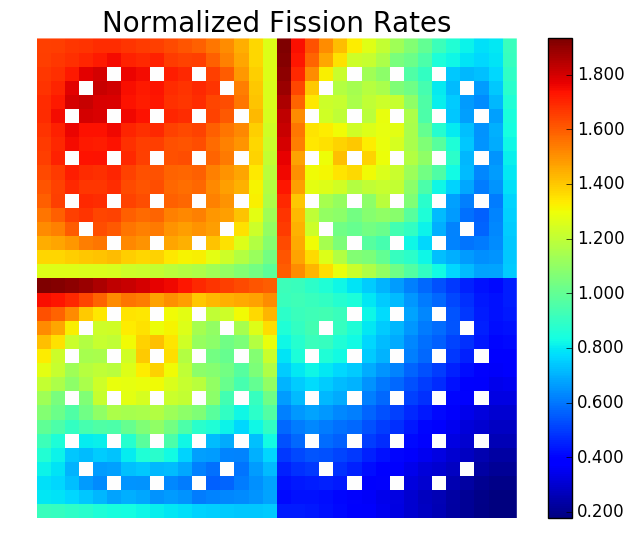
\includegraphics[width=0.8\linewidth]{figures/reflector/fission-rates}
  \caption{}
  \label{fig:fiss-reflector}
\end{subfigure}%
\begin{subfigure}{0.4\textwidth}
  \centering
  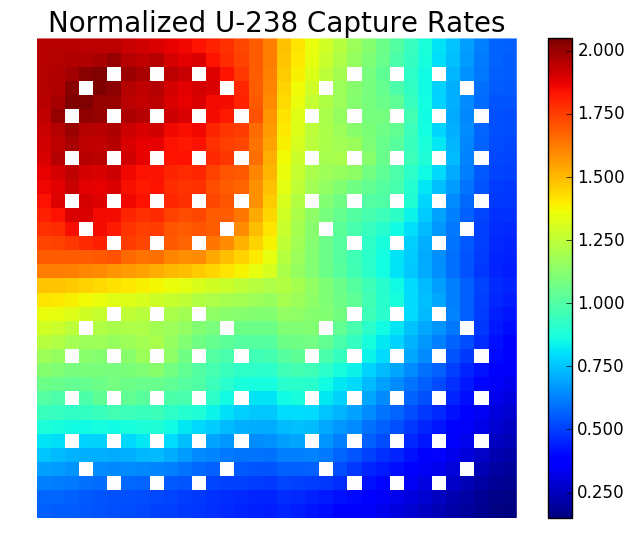
\includegraphics[width=0.8\linewidth]{figures/reflector/capture-rates}
  \caption{}
  \label{fig:capt-reflector}
\end{subfigure}
\caption{Reference OpenMC fission and U-238 capture rates for the assembly (a) -- (b) and colorset (c) -- (d) benchmarks.}
\label{fig:fiss-capt-rates}
\end{figure*}

The reference energy-integrated fission and U-238 capture rate spatial distributions were computed using rectilinear, pin-wise tally meshes in OpenMC and are shown in~\autoref{fig:fiss-capt-rates}. The reaction rates were normalized to the mean of all non-zero reaction rates. The rates in the instrument tubes, CRGTs and BPs are all zero and are shaded in white. The 1-sigma uncertainties are less than 0.08\% in each pin for both benchmarks.

%The fission rates include fission from only U-235 and U-238 for the fresh PWR UO$_2$ fuel. 
%The reaction rates were volume-integrated across each fuel pin.

As illustrated in the figures, the reaction rate distributions are strongly dependent on the spatially heterogeneous features in each benchmark. For example, the CRGTs provide additional moderation and increase the fission and U-238 capture rates in nearby fuel pins. The presence of a reflector with a mixture of vacuum and reflective boundaries induces a tilt in the reaction rates across the assemblies in the colorset.

Although spatial heterogeneities generally have similar effects on both fission and U-238 capture rates, there are a few important differences to note. The U-238 capture rates in the assemblies are more sensitive than the fission rates to the spatial self-shielding induced by moderation in CRGTs. In addition, the capture rates in the colorset are more smoothly varying at the inter-assembly and assembly-reflector interfaces than the fission rates.
